\documentclass{beamer}
\usepackage{fancyhdr}
\usepackage{hyperref}
\usepackage{graphicx}
\usepackage[font=itshape]{quoting}
\usepackage{pgfplots}
\usepackage{float}
\usepackage{amsmath}
\usepackage{tikz}
\usepackage{listings}
\usepackage{xcolor}
\usepackage[font=itshape]{quoting}
\newcommand{\comment}[1]{}
\title{Neural Networks}
\author{Oliver Temple}
\begin{document}
\begin{frame}
\titlepage
\end{frame}

\begin{frame}
\begin{abstract}
    Now commonplace in todays world, neural networks are becoming increasingly popular. This paper will explore the basic concepts behind neural networks, their history, how they are used in the real world and how the most simple neural networks work at a low level. The paper will conclude by exploring how to code a neural network from scratch to recognize hand written digits from 0-9.

    Neural networks are complex computational models that have many uses. Every one of the numerous different types of neural networks each has its own pros and cons which suits it for one or another of many possible tasks including computer vision, classification and prediction. The structure of neural networks can vary dramatically for different models, allowing for a wide range of applications. The fluidity of neural network structure allows them to adapt to a wide range of tasks.
    
    % Activation functions, loss functions, number of layers and neurons are just a few of the structure parameters that can be changed to create a neural network that suits the problem.
\end{abstract}
\end{frame}

\begin{frame}
\frametitle{Introduction}
\framesubtitle{What is a neural network?}
\begin{figure}[h!]
    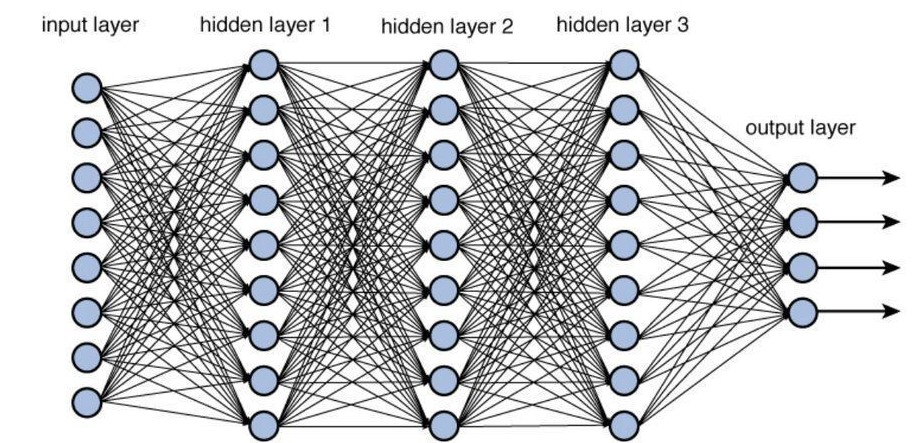
\includegraphics[width=\textwidth]{./assets/neural_network.jpeg}
    \caption{Neural Network}
    \label{fig:neural_network}
\end{figure}
\end{frame}

\begin{frame}
\frametitle{Introduction}
\framesubtitle{Different types of neural networks}
\begin{itemize}
    \item Perceptron
    \item Feed Forward Neural Network
    \item Multi-Layer Perceptron
    \item Convolutional Neural Network
    \item Recurrent Neural Network
    \item Long Short-Term Memory
\end{itemize} 
\end{frame}

\begin{frame}
\frametitle{Introduction}
\framesubtitle{Different types of neural networks}
All the different network types described below would of course be implemented in software, as part of a computer program. When modeling a neural network using software, it can have a number of different inputs $x_1, x_2, x_3 ... x_n$, which are assembled into a vector $\textbf{x}=\begin{bmatrix}x_1\\x_2\\x_3\\\vdots\\x_n\end{bmatrix}$. Likewise, the weights are also assembled into a vector (or a matrix in the case of more complicated models) $\textbf{W}=\begin{bmatrix}w_1\\w_2\\w_3\\\vdots\\w_n\end{bmatrix}$ or $\textbf{W}=\begin{bmatrix}w_{11}&w_{12}&w_{13}&\dots&w_{1n}\\w_{21}&w_{22}&w_{23}&\dots&w_{2n}\\w_{31}&w_{32}&w_{33}&\dots&w_{3n}\\\vdots&\vdots&\vdots&\ddots&\vdots\\w_{n1}&w_{n2}&w_{n3}&\dots&w_{nn}\end{bmatrix}$.
\subsubsection{Perceptron}
A perceptron model, often referred to as a neuron, shown in Figure~\ref{fig:perceptron}, is one of the simplest and oldest neural networks. It is the smallest unit of a neural network. It accepts inputs ranging between 0 and 1, and uses the weight that each connection has to calculate the output of the neuron by taking the vector dot product (Equation~\ref{eq:vector-dot-product}) of the weights and the inputs:
\begin{equation}
    \textbf{y} = \sigma(\textbf{W}\cdot\textbf{x} + b)
    \label{eq:perceptron}
\end{equation}
\end{frame}

\begin{frame}
\frametitle{Different types of neural networks}
\framesubtitle{Perceptron}
Where $\textbf{y}$ is the output, $\textbf{W}$ is a vector of the weights, $\textbf{x}$ is a vector of the inputs, $b$ is the bias and $\sigma$ is the activation function.
\end{frame}

\begin{frame}
\frametitle{Different types of neural networks}
\framesubtitle{Perceptron}
\begin{figure}[h!]
    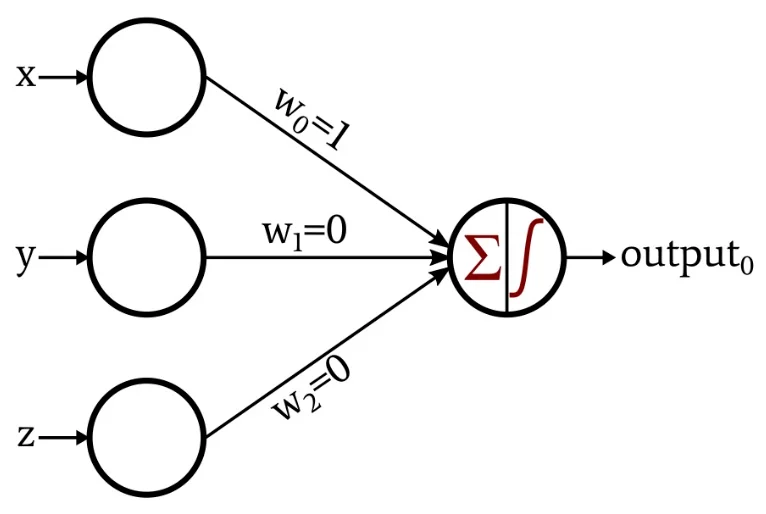
\includegraphics[width=\textwidth]{./assets/perceptron.png}
    \caption{Perceptron}
    \label{fig:perceptron}
\end{figure}
\end{frame}

\begin{frame}
\frametitle{Different types of neural networks}
\framesubtitle{Feed Forward Neural Network}
\begin{equation}
    \textbf{y}_n=\sigma{(\textbf{W}_n\cdot\textbf{y}_{n-1} + \textbf{b}_n)}
    \label{eq:feed-forward}
\end{equation}
\end{frame}

\begin{frame}
\frametitle{Different types of neural networks}
\framesubtitle{Feed Forward Neural Network}
Where $\textbf{y}_n$ is the output vector of the nth layer, $\textbf{W}_n$ is the weight matrix of the nth layer, $\textbf{y}_{n-1}$ is the output vector of the previous layer, $\textbf{b}_n$ is the bias vector of the nth layer, and $\sigma$ is the activation function.
\end{frame}

\begin{frame}
\frametitle{Different types of neural networks}
\framesubtitle{Convolutional Neural Network}
\begin{figure}[h!]
    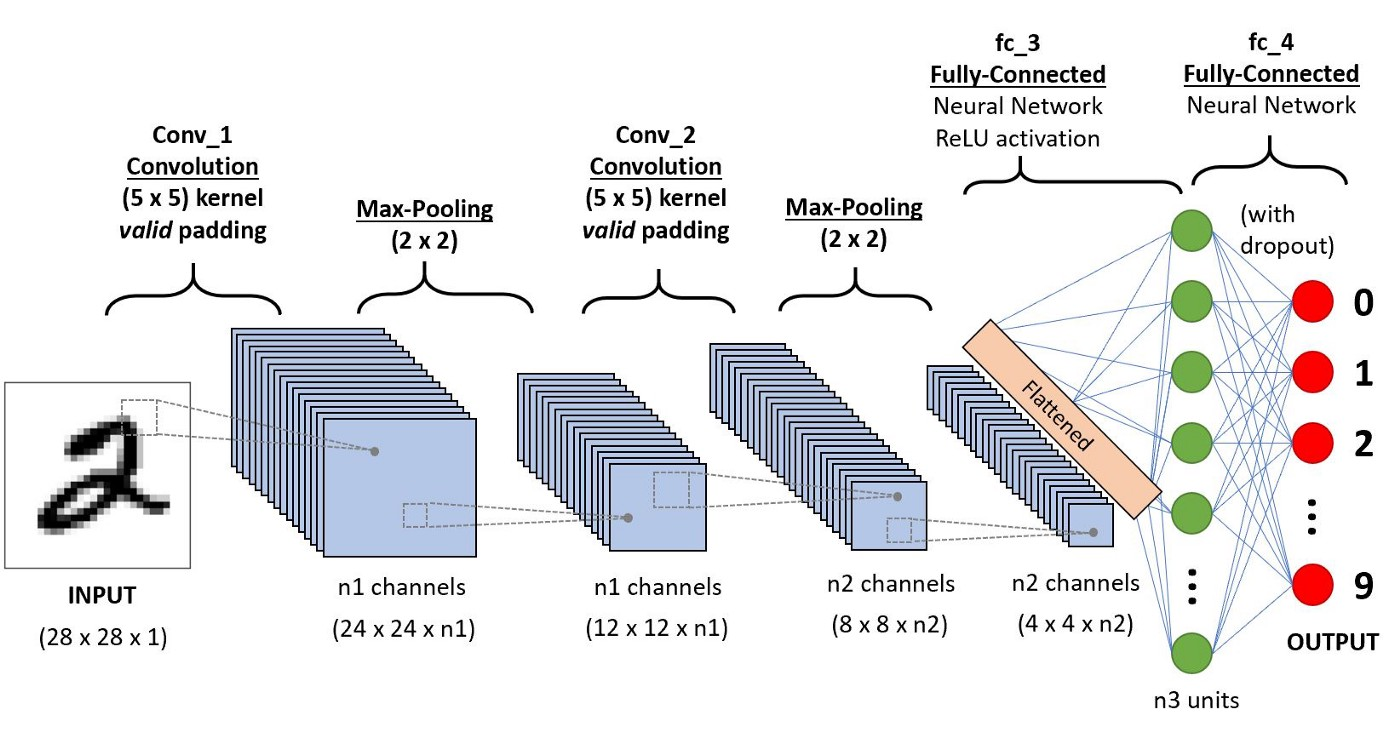
\includegraphics[width=\textwidth]{./assets/convolutional2.jpeg}
    \caption{Convolutional Neural Network}
    \label{fig:convolutional_neural_network}
\end{figure}
\end{frame}

\begin{frame}
\frametitle{The History of Neural Networks}
\framesubtitle{}
\begin{equation} \label{eq:Widrow-Hoff}
    \texttt{Weight Change} = \texttt{Pre-Weight line value}\times \frac{\texttt{Error}}{\texttt{Number of Inputs}}
\end{equation}
\end{frame}

\begin{frame}
\frametitle{Examples of Bias in AI}
\framesubtitle{PortraitAI Art Generator}
\begin{quoting}
    Currently, the AI portrait generator has been trained mostly on portraits of people of European ethnicity. We're planning to expand our dataset and fix this in the future. At the time of conceptualizing this AI, authors were not certain it would turn out to work at all. This generator is close to the state-of-the-art in AI at the moment. Sorry for the bias in the meanwhile. Have fun!
\end{quoting}
\end{frame}

\begin{frame}
\frametitle{Examples of Bias in AI}
\framesubtitle{Twitter Photo Cropping}
\begin{quoting}
    Our team did test for bias before shipping the model and did not find evidence of racial or gender bias in our testing. But it's clear from these examples that we've got more analysis to do. We'll continue to share what we learn, what actions we take, and will open source our analysis so others can review and replicate.
\end{quoting}
\end{frame}

\begin{frame}
\frametitle{How Neural Networks Work}
\framesubtitle{}
\begin{figure}[h!]
    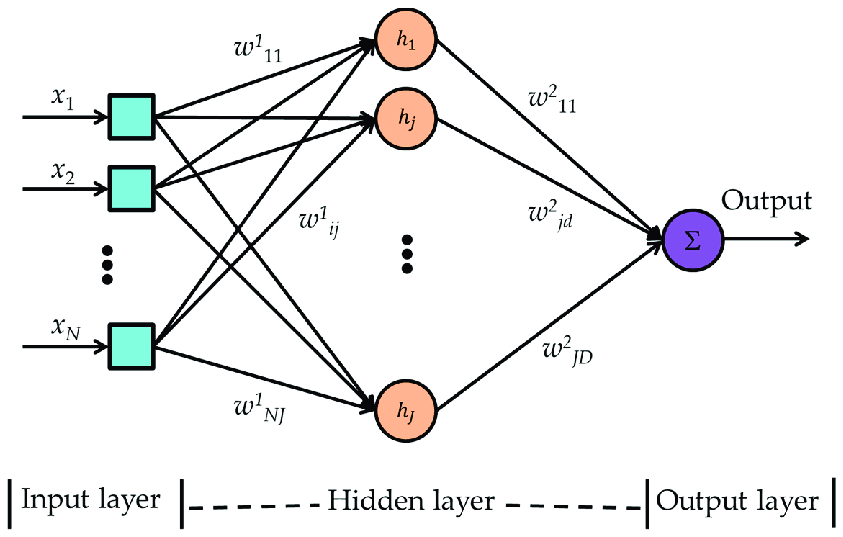
\includegraphics[width=\textwidth]{assets/multilayer perceptron.png}
    \caption{Multilayer Perceptron}
    \label{fig:multilayer-perceptron}
\end{figure}
\end{frame}

\begin{frame}
\frametitle{How Neural Networks Work}
\framesubtitle{Forward Propagation}
The purpose of forward propagation is to get an output (or prediction) from our neural network. To calculate it we use the vector dot product (Appendix~\ref{eq:vector-dot-product}) of the inputs and the weights, and add the bias. The output of the $n^{th}$ layer can be calculated using the formula in the equation~\ref{eq:forward-propagation}.
\end{frame}

\begin{frame}
\frametitle{How Neural Networks Work}
\framesubtitle{Forward Propagation}
\begin{equation}
    \textbf{y}_n = \sigma{(\textbf{W}_n\cdot\textbf{y}_{(n-1)} + \textbf{b}_n)}
    \label{eq:forward-propagation}
\end{equation}
\end{frame}

\begin{frame}
\frametitle{How Neural Networks Work}
\framesubtitle{Forward Propagation}
where $\textbf{W}_n$ is a matrix of the weights for the $n^{th}$ layer, $\textbf{y}_{(n-1)}$ is the output vector of the previous layer (the input of the network for the fist layer) and $\textbf{b}_n$ is a vector of the biases for the $n^{th}$ layer.
\end{frame}

\begin{frame}
\frametitle{How Neural Networks Work}
\framesubtitle{Activation Functions}
\begin{itemize}
    \item Sigmoid
    \item Tanh
    \item ReLU
    \item Leaky ReLU
\end{itemize}
\end{frame}

\begin{frame}
\frametitle{Activation Functions}
\framesubtitle{Sigmoid}
The sigmoid function(Figure~\ref{fig:sigmoid_function}) takes any input, $x$ and translates it to a value between 0 and 1. The equation is:
\end{frame}

\begin{frame}
\frametitle{Activation Functions}
\framesubtitle{Sigmoid}
\begin{equation}
    \sigma(x) = \frac{1}{1 + e^{-x}}
    \label{eq:sigmoid}
\end{equation}
\end{frame}

\begin{frame}
\frametitle{Activation Functions}
\framesubtitle{Sigmoid}
\begin{figure}[h!]
    \begin{center}
        \begin{tikzpicture}
            \begin{axis}[axis x line=bottom, axis y line=middle, xmin=-6, xmax=6, xlabel={$x$}, ylabel={$\sigma(x)$}]
            \addplot[color=red]{1/(1+exp(-x))};
            \end{axis}
        \end{tikzpicture}
    \end{center}
\end{figure}
\end{frame}

\begin{frame}
\frametitle{Activation Functions}
\framesubtitle{Tanh}
Similar to the sigmoid function, the tanh function(Figure~\ref{fig:tanh}) takes any input, $x$ and translates it to a value between -1 and 1. The equation is:
\end{frame}

\begin{frame}
\frametitle{Activation Functions}
\framesubtitle{Tanh}
\begin{equation}
    \tanh(x) = \frac{e^{x} - e^{-x}}{e^{x} + e^{-x}}
    \label{eq:tanh}
\end{equation}
\end{frame}

\begin{frame}
\frametitle{Activation Functions}
\framesubtitle{Tanh}
\begin{figure}[h!]
    \begin{center}
        \begin{tikzpicture}
            \begin{axis}[axis x line=bottom, axis y line=middle, xmin=-6, xmax=6, xlabel={$x$}, ylabel={$\tanh(x)$}]
            \addplot[color=red]{tanh(x)};
            \end{axis}
        \end{tikzpicture}
    \end{center}
\end{figure}
\end{frame}

\begin{frame}
\frametitle{Activation Functions}
\framesubtitle{ReLU}
Unlike the sigmoid function and the $\tanh$ function, the ReLU function(Figure~\ref{fig:relu}) takes any input, $x$ and if it is negative, it returns 0, otherwise it returns the input. The equation is:
\end{frame}

\begin{frame}
\frametitle{Activation Functions}
\framesubtitle{ReLU}
\begin{equation}
    \texttt{ReLU}(x) = \max(0, x)
    \label{eq:relu}
\end{equation}
\end{frame}

\begin{frame}
\frametitle{Activation Functions}
\framesubtitle{ReLU}
\begin{figure}[h!]
    \begin{center}
        \begin{tikzpicture}
            \begin{axis}[axis x line=bottom, axis y line=middle, xmin=-6, xmax=6, xlabel={$x$}, ylabel={$\texttt{ReLU}(x)$}]
            \addplot[color=red]{max(0, x)};
            \end{axis}
        \end{tikzpicture}
    \end{center}
\end{figure}
\end{frame}

\begin{frame}
\frametitle{Activation Functions}
\framesubtitle{Leaky ReLU}
The Leaky ReLU function(Figure~\ref{fig:leaky-relu}) takes any input, $x$ and if it is negative, it returns a scaled down input, otherwise it returns the input. The equation is:
\end{frame}

\begin{frame}
\frametitle{Activation Functions}
\framesubtitle{Leaky ReLU}
\begin{equation}
    \texttt{Leaky ReLU}(x) = \max(0.1x, x)
    \label{eq:leaky-relu}
\end{equation}
\end{frame}

\begin{frame}
\frametitle{Activation Functions}
\framesubtitle{Leaky ReLU}
\begin{figure}[h!]
    \begin{center}
        \begin{tikzpicture}
            \begin{axis}[axis x line=middle, axis y line=middle, xmin=-6, xmax=6, xlabel={$x$}, ylabel={$\texttt{Leaky ReLU}(x)$}]
            \addplot[color=red]{max(0.1*x, x)};
            \end{axis}
        \end{tikzpicture}
    \end{center}
\end{figure}
\end{frame}

\begin{frame}
\frametitle{How Neural Networks Work}
\framesubtitle{Loss Function}
\begin{itemize}
    \item Mean Squared Error (MSE)
    \item Cross Entropy Loss (or Log Loss)
\end{itemize}
\end{frame}

\begin{frame}
\frametitle{Loss Function}
\framesubtitle{Mean Squared Error}
\begin{equation}
    \texttt{MSE} = \frac{1}{n} \sum_{i=1}^{n} (\hat{y}_i - y_i)^2
    \label{eq:MSE}
\end{equation}
\end{frame}

\begin{frame}
\frametitle{Loss Function}
\framesubtitle{Mean Squared Error}
where $n$ is the number of samples we are testing against, $y$ is the desired output of the network, and $\hat{y}$ is the actual output of the network.
\end{frame}

\begin{frame}
\frametitle{Loss Function}
\framesubtitle{Cross Entropy Loss}
\begin{equation}
    \texttt{CEL} = -\frac{1}{n}\sum_{i=1}^{n}(y_i\times\log(\hat{y}_i))
    \label{eq:CEL}
\end{equation}
\end{frame}

\begin{frame}
\frametitle{Loss Function}
\framesubtitle{Cross Entropy Loss}
where $n$ is the number of samples we are testing against, $y$ is the desired output of the network, and $\hat{y}$ is the actual output of the network.
\end{frame}

\begin{frame}
\frametitle{How Neural Networks Work}
\framesubtitle{Backpropagation}
\begin{figure}[h!]
    \begin{center}
        \begin{tikzpicture}
            \begin{axis}[axis x line=middle, axis y line=middle, xlabel={Weight}, ylabel={Loss}]
            \addplot[color=red]{x*x};
            \end{axis}
        \end{tikzpicture}
    \end{center}
\end{figure}
\end{frame}

\begin{frame}
\frametitle{How Neural Networks Work}
\framesubtitle{Training}
\begin{enumerate}
    \item Propagate all the values in the input layer through the network (Forward Propagation).
    \item Update the weights and biases of the network using the loss function (Back Propagation).
    \item Repeat until the accuracy of the network is satisfactory.
\end{enumerate}
\end{frame}

\begin{frame}
\frametitle{Defining the Model}
\framesubtitle{Activation Function}
\begin{equation}
    \sigma'(x) = x(1-x)
    \label{eq:sigmoid-derivative}
\end{equation}
\end{frame}

\begin{frame}
\frametitle{Coding a Neural Network}
\framesubtitle{Training the Model}
\begin{figure}[h!]
    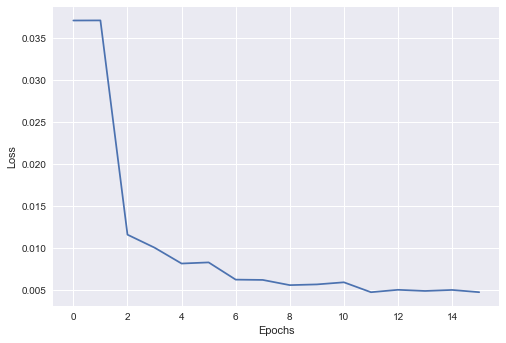
\includegraphics[width=\linewidth]{assets/loss.png}
    \caption{Loss of neural network over epochs}
    \label{fig:loss}
\end{figure}
\end{frame}

\begin{frame}
\frametitle{Training the Model}
\framesubtitle{The Curse of Dimensionality}
\begin{quotation}
    This phenomenon is known as the curse of dimensionality. Of particular concern is that the number of possible distinct configurations of a set of variables increases exponentially as the number of variables increases
\end{quotation}
\end{frame}

\begin{frame}
\frametitle{Coding a Neural Network}
\framesubtitle{Testing the Model}
\begin{figure}[h!]
    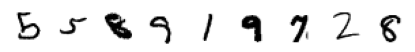
\includegraphics[width=\linewidth]{assets/sample_predictions.png}
    \caption{Sample predictions of neural network}
    \label{fig:sample-predictions}
\end{figure}
\end{frame}

\begin{frame}
\frametitle{Appendix}
\framesubtitle{Vector Dot Product}
    \begin{bmatrix}
        x_1\\
        x_2\\
        x_3\\
        \vdots\\
        x_n
    \end{bmatrix}
\end{frame}

\begin{frame}
\frametitle{Appendix}
\framesubtitle{Vector Dot Product}
    \begin{bmatrix}
        y_1\\
        y_2\\
        y_3\\
        \vdots\\
        y_n
    \end{bmatrix}
\end{frame}

\begin{frame}
\frametitle{Appendix}
\framesubtitle{Vector Dot Product}
    \begin{bmatrix}
        x_{11}&x_{12}&x_{13}&\dots&x_{1n}\\
        x_{21}&x_{22}&x_{23}&\dots&x_{2n}\\
        \vdots&\vdots&\vdots&\ddots&\vdots\\
        x_{n1}&x_{n2}&x_{n3}&\dots&x_{nn}
    \end{bmatrix}
\end{frame}

\begin{frame}
\frametitle{Appendix}
\framesubtitle{Vector Dot Product}
    \begin{bmatrix}
        y_1\\
        y_2\\
        \vdots\\
        y_n
    \end{bmatrix}
\end{frame}

\begin{frame}
\frametitle{Appendix}
\framesubtitle{Vector Dot Product}
    \begin{bmatrix}
        x_{11}y_1+x_{12}y_2+\dots+x_{1n}y_n\\
        x_{21}y_1+x_{22}y_2+\dots+x_{2n}y_n\\
        \vdots\\
        x_{n1}y_1+x_{n2}y_2+\dots+x_{nn}y_n
    \end{bmatrix}
\end{frame}

\begin{frame}
\frametitle{Appendix}
\framesubtitle{MNIST Dataset}
\begin{center}
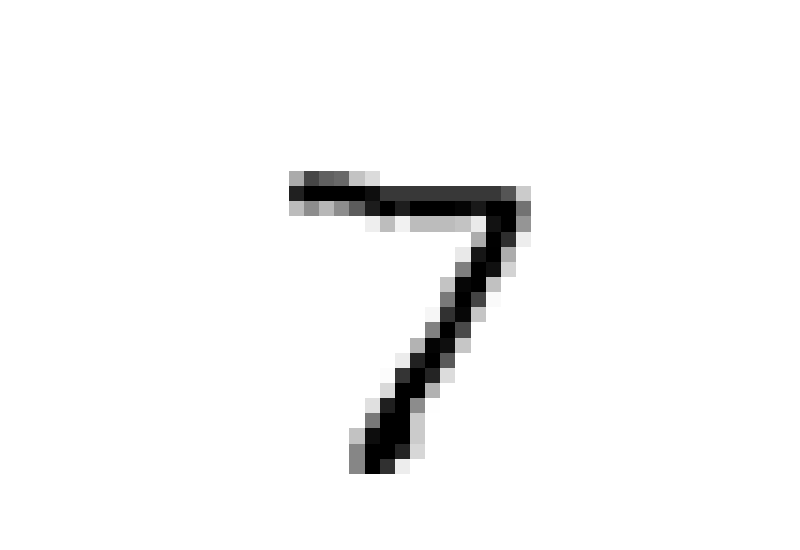
\includegraphics[width=\linewidth]{assets/mnist_example.png}
\end{center}
\end{frame}

\begin{frame}
\frametitle{Appendix}
\framesubtitle{MNIST Dataset}
\resizebox{\textwidth}{!}{
\begin{tabular}{c||c c c c c c c c c c}
    output & 1.3e-05 & 3.4e-06 & 0.0025 & 0.0025 & 7.9e-09 & 0.00033 & 2.9e-06 & \textbf{0.99} & 0.00062 & 2.5e-05 \\
    prediction & 0 & 1 & 2 & 3 & 4 & 5 & 6 & \textbf{7} & 8 & 9 \\
\end{tabular}}
\end{frame}

\begin{frame}
\frametitle{Appendix}
\framesubtitle{Python 3.9.10 Code}
\begin{thebibliography}{9}
    \bibitem{History of Neural Networks}
    \texttt{History of Neural Networks}
    \url{https://towardsdatascience.com/a-concise-history-of-neural-networks-2070655d3fec}
    \url{https://cs.stanford.edu/people/eroberts/courses/soco/projects/neural-networks/History/history1.html}
   
    \bibitem{Bias in Artificial Intelligence}
    \texttt{Bias in Artificial Intelligence}
    \url{https://www.lexalytics.com/lexablog/bias-in-ai-machine-learning}

    \bibitem{Loss Functions}
    \texttt{Loss Functions}
    \url{https://towardsdatascience.com/understanding-the-3-most-common-loss-functions-for-machine-learning-regression-23e0ef3e14d3}

    \bibitem{AI-hypotheses}
    \texttt{AI generated hypotheses}
    \url{https://www.scientificamerican.com/article/ai-generates-hypotheses-human-scientists-have-not-thought-of/}

    \bibitem{curse-of-dimensionality}
    \texttt{Curse of dimensionality}
    Page 155, Deep Learning (Adaptive Computation and Machine Learning series) by Yoshua Bongio and Aaron Courville

    \bibitem{3Blue1Brown Neural Networks}
    \texttt{3Blue1Brown Neural Networks}
    \url{https://www.youtube.com/playlist?list=PLZHQObOWTQDNU6R1_67000Dx_ZCJB-3pi}

    \bibitem{convolutionalnn}
    \texttt{Convolutional Neural Networks}
    \url{https://towardsdatascience.com/a-comprehensive-guide-to-convolutional-neural-networks-the-eli5-way-3bd2b1164a53}

    \bibitem{vonneumann}
    \texttt{Von Neumann Architecture}
    \url{https://en.wikipedia.org/wiki/Von_Neumann_architecture}

    \bibitem{tensorflow}
    \texttt{TensorFlow}
    \url{https://www.tensorflow.org/resources/learn-ml?gclid=Cj0KCQiA64GRBhCZARIsAHOLriIX8Z76A8AJhOpEWU0Nl9PMrZ5kUqc4DUuybvBHsAmIhz0OeBNlyYoaAmezEALw_wcB}

    \bibitem{pytorch}
    \texttt{PyTorch}
    \url{https://pytorch.org/}
\end{thebibliography}
\end{frame}
\end{document}
